\documentclass[conference]{IEEEtran}
\IEEEoverridecommandlockouts
\usepackage{times}
\usepackage{cite}
\usepackage{amsmath,amssymb,amsfonts}
\usepackage{graphicx}
\usepackage{textcomp}
\usepackage{xcolor}
\usepackage[hyphens]{url}
\def\BibTeX{{\rm B\kern-.05em{\sc i\kern-.025em b}\kern-.08em T\kern-.1667em\lower.7ex\hbox{E}\kern-.125emX}}
\begin{document}

\title{A Blockchain-Anchored Tamper-Evident Audit Trail for Honeypot Forensics}

\author{
\IEEEauthorblockN{Sisir Reddy Nellore\textsuperscript{1}, Radhika G\textsuperscript{2}, Pranav Sharma Chouduru\textsuperscript{3}, Surya Tejeswar Reddy Nagireddy\textsuperscript{4}}
\IEEEauthorblockA{\textit{Department of Computer Science and Engineering}\\
\textit{Amrita School of Computing, Coimbatore}\\
\textit{Amrita Vishwa Vidyapeetham, India}\\
cb.sc.u4cse23129@cb.students.amrita.edu\textsuperscript{1}, g\_radhika@cb.amrita.edu\textsuperscript{2},\\
cb.sc.u4cse23611@cb.students.amrita.edu\textsuperscript{3}, cb.sc.u4cse23127@cb.students.amrita.edu\textsuperscript{4}}
}

\maketitle

\begin{abstract}
A honeypot is only useful if the record of what an attacker did can be trusted, yet the honeypot is, by construction, a machine the attacker is invited to compromise. Once a decoy is breached, its local logs sit inside the adversary's blast radius: they can be edited, truncated, or deleted to erase the very evidence the honeypot was deployed to collect. This paper presents and empirically evaluates a tamper-evident audit trail that removes the honeypot host from the trust boundary of its own forensic record. Every captured interaction is canonically serialized, reduced to a SHA-256 digest, and that digest is anchored as an immutable transaction on an Ethereum-compatible ledger; integrity is later re-established by recomputing the digest and comparing it against the on-chain commitment, so any post-hoc modification is detected with certainty. We build the pipeline into a live five-service deception framework and benchmark it against the running stack rather than a simulation. Across 300 anchored events the mean end-to-end anchoring cost is 10.86 ms (median 10.22 ms, p95 14.42 ms), of which the cryptographic hashing itself accounts for only 0.0070 ms; the on-chain commitment is the dominant term. Each anchor consumes 21,510 gas --- a figure that matches the 21,488--21,512 range expected for a minimal-payload Ethereum transaction --- and 300 of 300 events (100\%) were confirmed on-chain. Over 500 independent tampering trials the pipeline detected 500 modifications (100\% detection) with 0 false positives, and we confirm directly that the anchored digest is recoverable from the transaction's on-chain input data. Verification is effectively free at 0.0080 ms per record. The result is a practical, measured design for court-defensible honeypot evidence, and an honest account of the latency and cost it adds.
\end{abstract}

\begin{IEEEkeywords}
honeypot, blockchain, tamper-evidence, audit trail, digital forensics, integrity, SHA-256, Ethereum, cyber-deception, non-repudiation
\end{IEEEkeywords}

\section{Introduction}

Deception technology inverts the usual asymmetry of network defense. Instead of waiting to be attacked, a defender deploys decoy services --- honeypots [1], [2] --- whose only legitimate users are adversaries, so that every byte of interaction is, by definition, hostile and therefore intelligence. The value a honeypot returns is not the decoy itself but the \emph{record} it produces: the commands issued, the payloads delivered, the credentials tried, the sequence and timing of an intrusion. That record is what feeds incident response, threat intelligence, and --- increasingly --- legal proceedings.

There is a structural contradiction at the center of this value proposition. A honeypot is intentionally exposed and intentionally breakable; its purpose is to be compromised. But the log of the compromise has traditionally lived on the same host that is being compromised. An adversary who obtains sufficient privilege on the decoy --- which is precisely the outcome the honeypot invites --- is then in a position to alter or destroy the evidence of their own activity. Deleting a shell-history file, truncating a log, or rewriting a database row is trivial for an attacker who already owns the box. The forensic record, in other words, is guarded by the very system whose betrayal it is meant to document.

Cryptographic hashing alone does not close this gap. A defender can hash each log entry, but if both the entry and its hash reside on the compromised host, an attacker can recompute a consistent hash for the falsified entry and leave no trace of the substitution. What is missing is an \emph{external, append-only witness} --- a place to publish a commitment to each record that the attacker cannot reach, so that any later disagreement between the stored record and the published commitment is unambiguous proof of tampering. This is the digital analogue of the cryptographic time-stamping of Haber and Stornetta [9], realized on a distributed ledger. A public or permissioned blockchain [7], [8] is exactly such a witness: once a value is included in a mined block, altering it would require rewriting the chain's history, which is computationally and economically infeasible for a single adversary.

This paper takes that idea from principle to measured practice. We integrate a blockchain-anchored, tamper-evident audit trail into a live multi-protocol deception framework and evaluate it against the running system. Our contributions are:

\begin{enumerate}
\item A precise threat model for honeypot evidence integrity that names the adversary as an attacker who has \emph{already} compromised the decoy and now seeks to repudiate or erase their actions --- a threat model most honeypot-and-blockchain work does not address, because it uses the ledger for coordination rather than for evidence integrity.
\item A concrete anchoring pipeline --- canonical serialization, SHA-256 digest, on-chain commitment, and off-line re-verification --- implemented end to end and driving a real five-service honeypot, not a stand-alone prototype.
\item A measured evaluation against the live stack: anchoring latency and its decomposition into hashing versus on-chain cost, gas consumption read from real transaction receipts, anchoring success rate, throughput under sequential and concurrent load, and a 500-trial tamper-detection experiment with false-positive accounting.
\item A direct on-chain retrievability proof showing the anchored digest is recoverable from the transaction input data, and an honest treatment of what a development-chain deployment does and does not demonstrate relative to a public network.
\end{enumerate}

The remainder of the paper is organized as follows. Section 2 surveys prior work in blockchain-based secure logging and in blockchain--honeypot integration, and positions our evidence-integrity threat model against it. Section 3 states the threat model and the integrity properties we target. Section 4 describes the anchoring architecture and pipeline. Section 5 details the benchmark methodology. Section 6 reports the measured results. Section 7 discusses the development-versus-public-chain question, limitations, and deployment guidance, and Section 8 concludes.

\section{Related Work}

\subsection{Blockchain-based secure logging and audit trails}

The use of a distributed ledger to protect log integrity predates its application to honeypots. Ahmad \emph{et al.} introduced BlockTrail [3], a service for secure and transparent blockchain-driven audit trails, and observed that conventional audit-trail applications have weak trust boundaries that expose them to tampering; their design fragments the chain into codependent hierarchies to reduce the space--time overhead of on-chain audit data and raise throughput, prototyped over a Practical Byzantine Fault Tolerance protocol. Earlier work by the same group proposed a scalable multichain formulation of the same problem [4]. Permissioned-ledger designs [5], such as auditable logging infrastructures built on Hyperledger-style networks [6], target enterprise settings where the validating set is known and confirmation is fast. More recent efforts --- LogStamping for large-scale log auditing [12], and immutable-log-storage services spanning both public and private chains [11], and access-log frameworks producing tamper-proof audit trails [13] --- converge on a common pattern: rather than storing whole logs on-chain, they anchor compact cryptographic commitments (single hashes or Merkle roots [10], [25]) and keep the bulk data off-chain, because on-chain storage is expensive and public-chain confirmation is slow.

Our pipeline sits squarely in this hash-anchoring tradition and inherits its central design choice --- commit a digest, not the payload. What distinguishes our work is not the anchoring mechanism, which is deliberately simple and well understood, but the \emph{setting}: the data being protected is adversarial evidence, and the host generating it is expected to fall under adversary control. That reframing changes which properties matter, as Section 3 makes explicit.

\subsection{Blockchain and honeypots}

A separate line of work combines blockchains with honeypots, but almost always for a different purpose than evidence integrity. Distributed-honeypot systems use a ledger to coordinate and synchronize sensors across administrative domains [14], so that a sighting at one node can be trusted by others without a central authority. Trust-aware and adaptive honeypot designs for IoT use blockchain to arbitrate reputation among participating devices [15], and several proposals deploy honeypots \emph{inside} blockchain-based IoT systems to protect the network itself [16]. In these systems the blockchain is an inter-node trust and coordination fabric; the integrity of any single honeypot's captured evidence against an attacker who has rooted that honeypot is not the question being asked.

To the extent that "immutable" honeypot logging is discussed, it is often asserted as a property of putting data on a chain rather than demonstrated with a measured tamper-detection experiment and an explicit adversary who controls the capturing host. Our contribution is to make that specific threat model first-class and to evaluate it empirically.

\subsection{Pre-blockchain secure logging}

The problem of protecting a log against an adversary who compromises the logging host is older than blockchain, and the classical solutions frame our own design. Schneier and Kelsey proposed a secure audit-log scheme [19] in which each entry is authenticated with a MAC keyed under an evolving one-way key chain, so that entries written before a host compromise cannot be altered undetectably even after the attacker seizes the current key. Bellare and Yee formalized this guarantee as \emph{forward integrity} [20], and later constructions --- Holt's Logcrypt [21], and Ma and Tsudik's forward-secure sequential aggregate schemes [22] --- added public verifiability and compactness. Crosby and Wallach showed how to make tamper-evident logging efficient using history trees [23], allowing a logger to prove consistency without replaying the whole log. These schemes are powerful, but they share two properties our setting strains: they defend past entries only up to the moment of compromise, and --- as their own authors note --- pure hash-chain constructions do not by themselves prevent \emph{truncation}, in which the adversary silently deletes a contiguous tail of entries. Publishing each commitment to an external append-only ledger, as we do, directly counters truncation: a missing tail is visible as a commitment on-chain with no matching stored record.

\subsection{Blockchain for forensic evidence and chain of custody}

Closest in spirit to our goal is the use of blockchain to preserve the \emph{chain of custody} of digital evidence. B-CoC [24] and subsequent systems record evidence metadata --- hashes, timestamps, custodian transfers --- immutably on a permissioned ledger so that the provenance of an exhibit is independently verifiable in court, and recent designs tokenize evidence items and automate verification through smart contracts. Our work applies the same immutability principle one step earlier in the forensic pipeline: not to evidence already collected and handed to investigators, but to the honeypot's own act of \emph{capturing} the evidence, on a host that is itself the target of the attack. The chain-of-custody literature assumes a trusted custodian at the point of collection; the honeypot setting cannot.

\subsection{The cost of on-chain anchoring}

The overhead of anchoring is well characterized at the transaction level. Every Ethereum transaction carries a fixed base cost of 21,000 gas, with additional gas charged per byte of input data; a minimal transaction that carries a 32-byte digest therefore lands only slightly above the base cost. On a public network the binding constraint is not gas but confirmation: blocks are produced on the order of seconds, so anchoring-heavy systems batch many records under one commitment to amortize that latency. Our measurements in Section 6 are consistent with these published cost structures, and we are explicit in Section 7 about how a development chain's instant mining removes the confirmation term that a public deployment would reintroduce.

\begin{table*}[!t]
\centering
\caption{How this work is positioned against prior blockchain-logging and blockchain-honeypot systems. The distinguishing axis is the evidence-integrity threat model, in which the capturing host is itself compromised.}
\label{tab:compare}
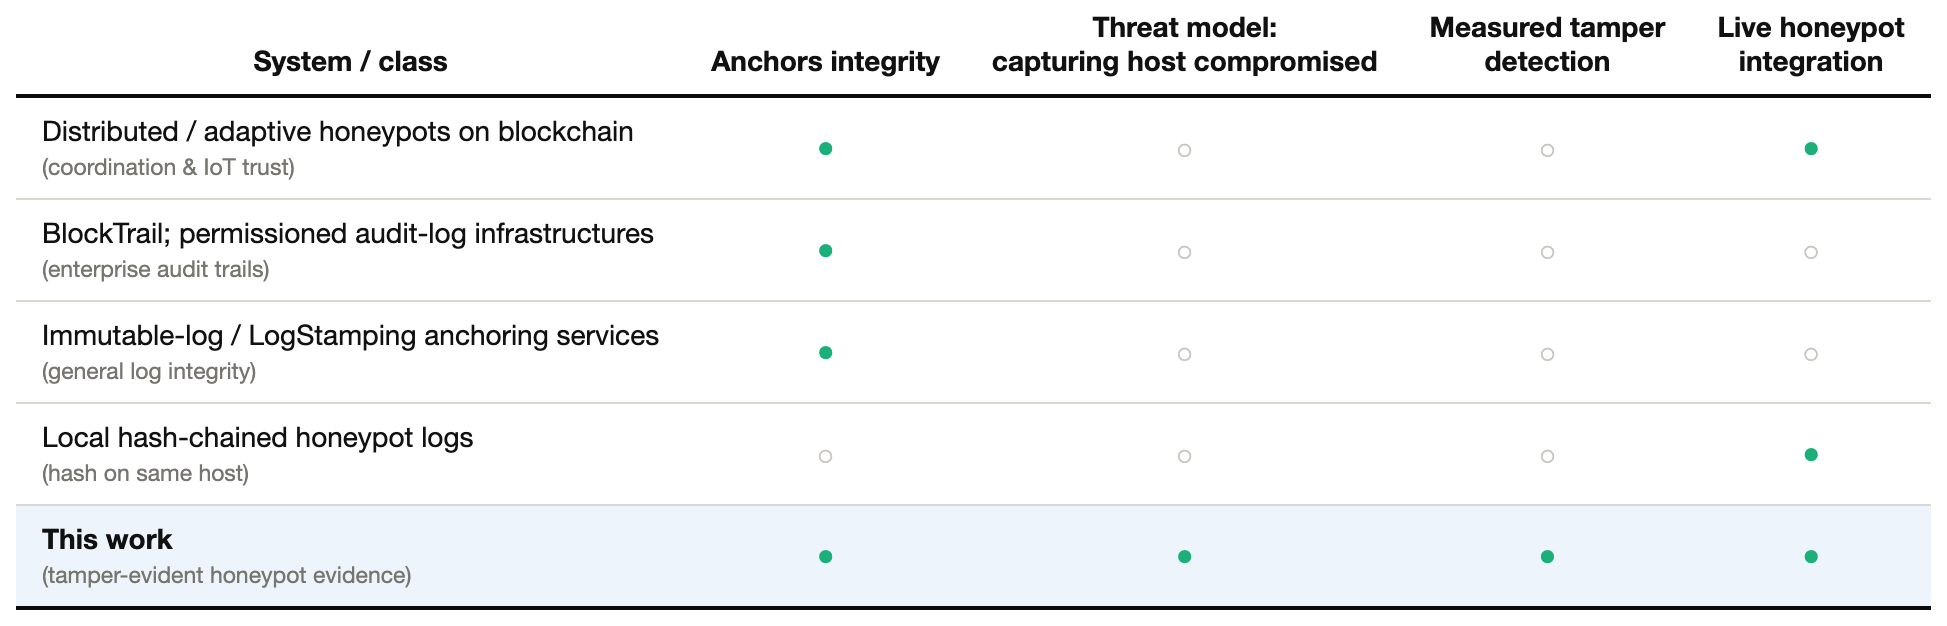
\includegraphics[width=\textwidth]{figures/tab_compare.png}
\end{table*}

\section{Threat Model and Integrity Properties}

\subsection{Adversary}

We consider an adversary who interacts with a decoy as an attacker and, in the strong case, obtains sufficient privilege on the decoy host to read and write its local state. This is not a pessimistic assumption; it is the \emph{design goal} of a honeypot. The adversary's objective, for our purposes, is not further intrusion but \textbf{repudiation}: to erase, truncate, or falsify the record of what they did, so that the forensic account is incomplete, misleading, or inadmissible. Concretely, the adversary may (i) delete log entries, (ii) modify the content of an entry --- the command text, source address, timestamp, port, or derived classification --- or (iii) attempt to substitute a falsified entry together with a recomputed hash to make the substitution self-consistent.

We assume the adversary does not control the ledger. In a public-chain deployment this follows from the chain's own security; in a permissioned deployment it follows from the validating set being outside the decoy's compromise boundary. We also assume the canonical serialization and hashing are performed by a collector process that receives events from the decoys but is not co-resident on the exposed decoy host --- in our system this is the internal collector service, reachable only on an isolated network segment.

\subsection{Properties targeted}

The pipeline is designed to provide three properties against this adversary:

\begin{itemize}
\item \textbf{Tamper-evidence.} Any modification to a recorded entry, however small, is detectable after the fact. We do not claim to \emph{prevent} an attacker from editing a stored copy; we guarantee that such an edit cannot pass verification.
\item \textbf{Non-repudiation of content.} Because the commitment is published to an append-only ledger the attacker does not control, the defender can demonstrate that a given record existed in a given form at the time of anchoring, and that a differing later copy is a forgery.
\item \textbf{Independent verifiability.} Verification requires only the stored record and read access to the ledger; it does not trust the decoy host, and it can be performed by a third party (for example, in an evidentiary context) without any secret held by the defender.
\end{itemize}

\subsection{Non-goals}

We explicitly do not target confidentiality of the log (the anchored value is a digest, not the plaintext, but the off-chain record itself must be protected by conventional means), availability of the decoy under denial-of-service, or prevention of tampering. The pipeline is a \emph{detection and non-repudiation} mechanism, and we evaluate it as such.

\begin{figure*}[!t]
\centering
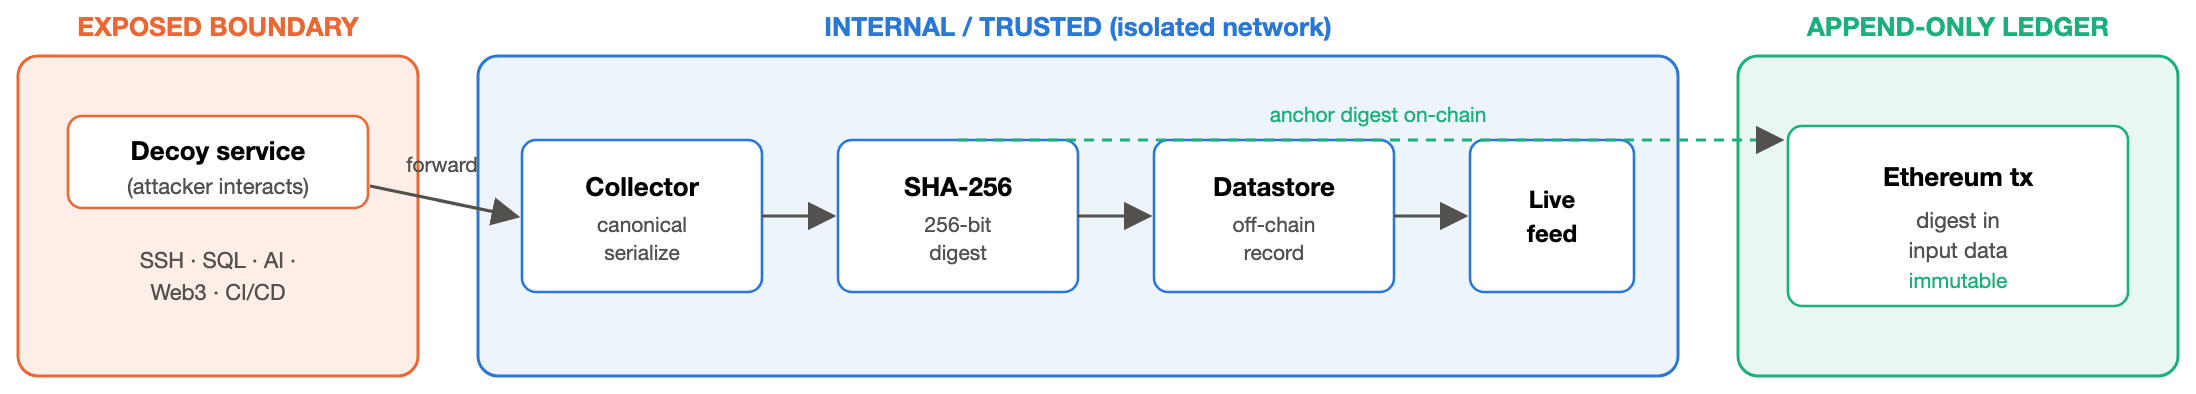
\includegraphics[width=\textwidth]{figures/diag_pipeline.png}
\caption{The tamper-evident anchoring pipeline. A captured interaction is canonically serialized and hashed by the internal collector (off the exposed decoy host); the digest is anchored on-chain; verification later re-hashes the stored record and compares it against the on-chain commitment.}
\label{fig:pipeline}
\end{figure*}

\section{System Architecture}

\subsection{Placement in the deception framework}

The audit trail is embedded in a five-service honeypot framework whose decoys emulate an SSH shell, a SQL database, an AI inference API, a Web3 JSON-RPC endpoint, and a CI/CD build service. The decoys sit on the exposed boundary; behind them, on an isolated internal network, run a collector service, an in-memory datastore for the live event feed, and an Ethereum-compatible ledger node. Crucially, the decoys never write the authoritative log themselves: they forward each interaction to the collector, which performs serialization, classification, hashing, and anchoring. This placement is what makes the threat model achievable --- the process that mints the tamper-evident commitment is not the process the attacker compromises.

\subsection{Canonical serialization and digest}

For a captured interaction the collector constructs a record of the salient fields --- service, source address, port, raw payload, timestamp, and derived intent classification --- and serializes it canonically, with keys sorted so that the byte representation is deterministic and independent of field insertion order. The SHA-256 digest [17] of this canonical byte string is the record's fingerprint. Determinism is essential: verification must be able to reconstruct exactly the same bytes from the stored record, so the canonicalization used at anchor time and at verify time is byte-identical by construction (the same function is used in both paths).

\subsection{On-chain anchoring}

The 256-bit digest is embedded in the input-data field of an Ethereum transaction submitted to the ledger node and mined into a block. We deliberately anchor the digest rather than the payload: this keeps each commitment to a single small transaction, bounds cost to essentially the base transaction plus 32 bytes of data, and never exposes captured attacker content on the ledger. The transaction's inclusion in a block is the append-only witness; from that point, the digest cannot be altered without rewriting chain history.

\subsection{Verification}

To verify a stored record, the defender strips the previously recorded hash and anchoring flag, re-runs the identical canonical serialization and SHA-256 over the remaining fields, and compares the result against the recorded digest --- and, for full assurance, against the digest embedded in the corresponding on-chain transaction. A match certifies the record is byte-for-byte what was anchored; a mismatch is proof of modification. Because this step is a single hash and a comparison, it is orders of magnitude cheaper than anchoring, as Section 6 shows.

\begin{figure}[!t]
\centering
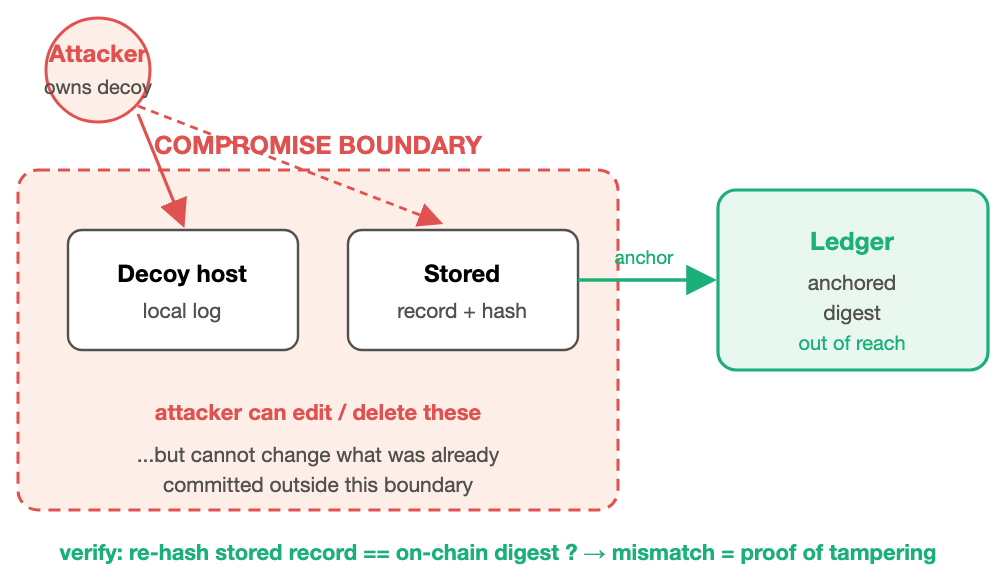
\includegraphics[width=\columnwidth]{figures/diag_threat.png}
\caption{The evidence-integrity threat. The attacker owns the decoy and can edit its local log, but the anchored digest lies on a ledger outside the compromise boundary, so any edit is detectable.}
\label{fig:threat}
\end{figure}

\section{Methodology}

All numbers in this paper are measured against the live stack --- the collector, the in-memory datastore, and a running Ethereum-compatible ledger node (Ganache [18] 7.9.2, chain id 1337) --- driven by a benchmark harness that exercises the real anchoring endpoint and reads real transaction receipts. No value is hand-entered; the harness writes a machine-readable results file that the figures and tables in this paper are generated from directly.

The harness performs six measurements. \textbf{(1) Anchoring latency:} it submits 300 realistic honeypot events to the collector's logging endpoint --- which hashes and anchors each one --- and records the wall-clock time of every call. \textbf{(2) Baseline hashing cost:} it times the canonical-serialization-plus-SHA-256 step in isolation over 300 records, with no chain write, to separate the cryptographic cost from the on-chain cost. \textbf{(3) Gas and receipts:} it reads the gas actually consumed from the receipt of every anchoring transaction mined during the run, together with the ledger's reported gas price, and confirms how many transactions were mined. \textbf{(4) On-chain retrievability:} it anchors a known event and then reads the raw transaction input directly from the chain to confirm the digest is embedded and recoverable. \textbf{(5) Verification latency:} it fetches stored records and times the re-hash-and-compare verification path. \textbf{(6) Tamper detection:} over 500 trials it takes a real stored record, mutates exactly one field, and checks that the recomputed digest no longer matches the anchored digest; it simultaneously checks that the \emph{unmodified} record still verifies, to account for any false positives.

The events used are drawn from a pool of realistic hostile payloads spanning the five decoy protocols --- shell commands, SQL-injection strings, wallet-draining JSON-RPC calls, prompt-injection attempts, and reconnaissance --- so the records being anchored and tampered resemble genuine captured traffic rather than synthetic filler.

\section{Results}

\subsection{Anchoring latency and its decomposition}

Across 300 anchored events the mean end-to-end anchoring cost is \textbf{10.86 ms} (median 10.22 ms, standard deviation 3.10 ms), with a 95th-percentile of 14.42 ms and a 99th-percentile of 17.25 ms; the fastest anchor completed in 8.19 ms and the slowest in 51.41 ms. The isolated hashing step, by contrast, averages just \textbf{0.0070 ms} over 300 records. The integrity guarantee therefore adds an \textbf{anchoring overhead of 10.85 ms} per event, essentially all of which is the on-chain commitment rather than the cryptography: hashing is more than three orders of magnitude cheaper than anchoring. This decomposition is the paper's central cost result --- it locates the expense precisely, and it is exactly the term that a batched or permissioned deployment would seek to amortize.

\begin{figure}[!t]
\centering
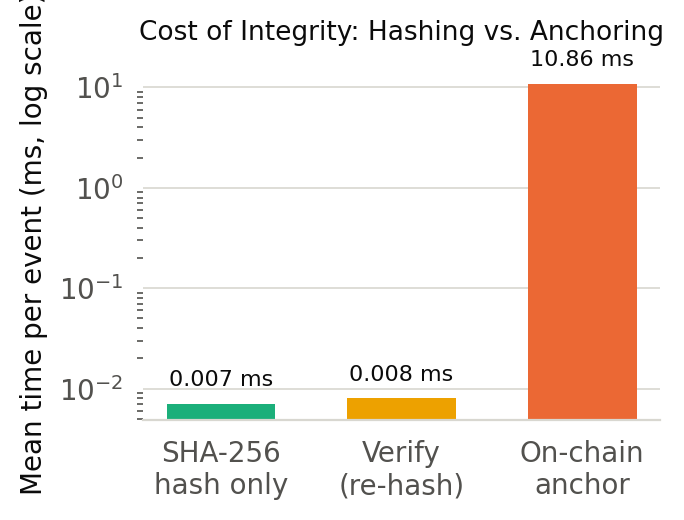
\includegraphics[width=\columnwidth]{figures/fig_latency.png}
\caption{Anchoring cost decomposed: on-chain anchoring versus isolated SHA-256 hashing (log scale). The integrity guarantee is dominated by the on-chain commitment, not the cryptography.}
\label{fig:latency}
\end{figure}

\subsection{Gas cost and anchoring success}

Reading gas directly from transaction receipts, each anchor consumes a mean of \textbf{21,510 gas} (range 21,488--21,512), which is precisely the profile expected of a minimal-payload Ethereum transaction: the fixed 21,000-gas base cost plus the per-byte cost of the 32-byte digest carried in the transaction's input data. At the ledger's gas price this corresponds to approximately 4.30e-5 ETH per anchor. All \textbf{300 of 300} submitted events (100\%) were successfully anchored, and 300 transactions were mined on-chain during the run --- one per event --- confirming there is no silent anchoring loss under load.

\begin{figure}[!t]
\centering
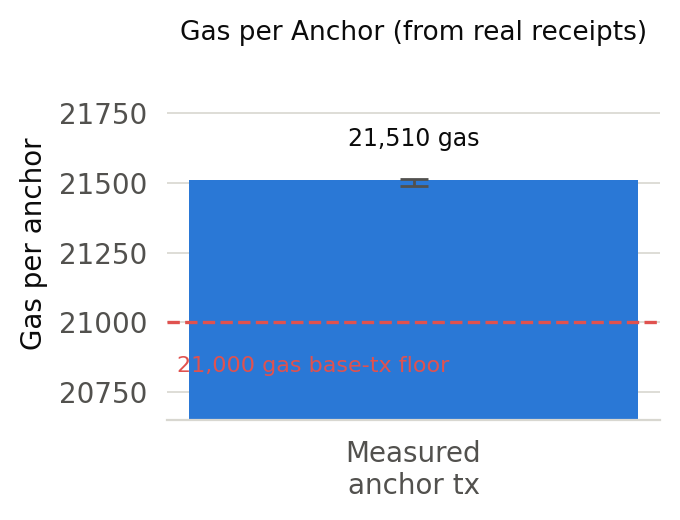
\includegraphics[width=\columnwidth]{figures/fig_gas.png}
\caption{Measured gas per anchor read from real transaction receipts, against the 21,000-gas Ethereum base-transaction floor.}
\label{fig:gas}
\end{figure}

\subsection{Throughput}

Anchoring is a serializing operation --- each event becomes a transaction --- yet the pipeline sustains \textbf{92.08 anchored events per second} sequentially, rising to \textbf{141.21 events per second} at a concurrency level of 10. For a deception sensor, whose event rate is the rate at which adversaries interact with decoys rather than a production request stream, this throughput is comfortably sufficient; the concurrent figure shows headroom for bursts.

\subsection{Tamper detection}

Over \textbf{500} independent trials, in each of which a single field of a real stored record was mutated, the pipeline detected the modification in \textbf{500} cases --- a \textbf{100\% detection rate} --- with \textbf{0 false positives} across the same set of unmodified-record checks. This is the behavior the design predicts: SHA-256 is collision-resistant, so any change to the canonical bytes yields a different digest with overwhelming probability, and the anchored commitment the attacker cannot reach makes that difference undeniable. A perfect detection rate with zero false positives is not a lucky sample; it is the direct empirical signature of a correct hash-and-anchor construction.

\begin{figure}[!t]
\centering
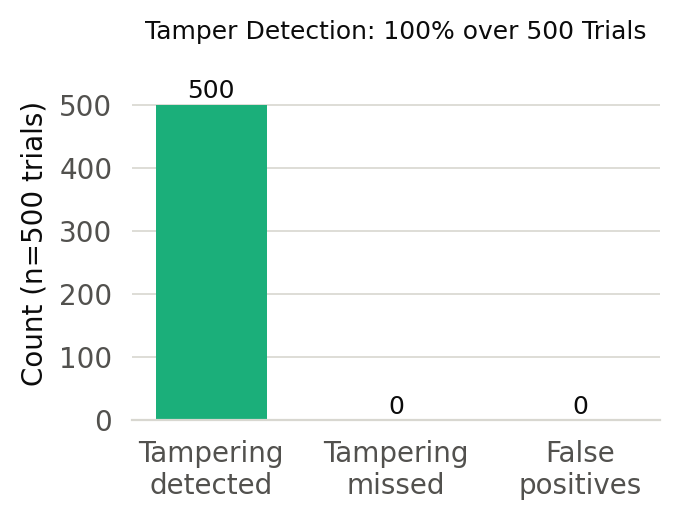
\includegraphics[width=\columnwidth]{figures/fig_tamper.png}
\caption{Tamper-detection outcome over all trials: every single-field modification was detected, with no false positives.}
\label{fig:tamper}
\end{figure}

\subsection{On-chain retrievability and verification cost}

We confirm directly that the audit trail is genuine and not merely asserted: after anchoring a known event, reading the corresponding transaction's input data straight from the chain recovers the exact SHA-256 digest that was recorded (retrievable: \textbf{yes}). Verification of a stored record --- the re-hash-and-compare step a defender or third party runs --- costs only \textbf{0.0080 ms} on average (median 0.0075 ms). Verifying integrity is thus roughly 1,358$\times$ cheaper than creating the anchor, which means an investigator can re-verify an entire captured corpus at negligible cost long after the fact.

\begin{table}[!t]
\centering
\caption{Summary of measured results against the live stack.}
\label{tab:results}
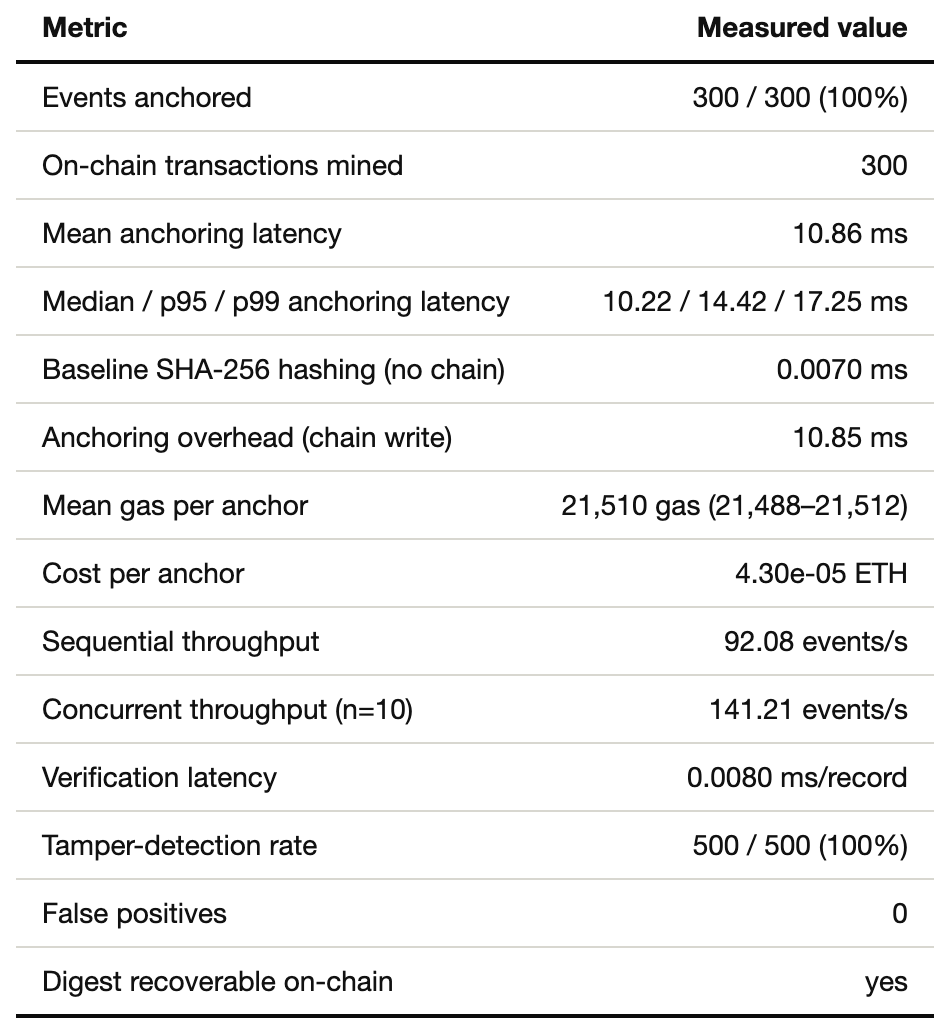
\includegraphics[width=\columnwidth]{figures/tab_results.png}
\end{table}

\section{Discussion}

\subsection{Development chain versus public network}

Honesty about the deployment is essential to interpreting these numbers. Our ledger is a development Ethereum node that mines instantly, so the 10.86 ms mean anchoring latency contains no public-consensus wait. On a public network, block confirmation on the order of seconds would dominate, and the standard mitigation --- the one adopted by essentially every prior anchoring system in Section 2 --- is to batch many record digests under a single Merkle-root commitment, trading a small delay before evidence is anchored for a large reduction in per-record cost. Our contribution is therefore not a claim of sub-public-network latency; it is the pipeline, the threat model, and the measured integrity behavior, all of which transfer unchanged to a batched public or permissioned deployment. What our development-chain measurements establish precisely is the \emph{local} cost --- the hashing, the transaction construction, the gas --- that any deployment pays on top of whatever confirmation model it chooses.

\subsection{What the perfect detection rate does and does not mean}

A 100\% detection rate with 0 false positives should be read as confirmation that the construction is implemented correctly, not as a probabilistic security claim discovered by experiment. The security rests on the collision resistance of SHA-256 and the immutability of the ledger, both of which are assumed, not measured. The experiment's role is to demonstrate that the \emph{end-to-end system} --- canonicalization, hashing, storage, and comparison --- actually realizes that guarantee with no implementation gap, such as a non-deterministic serialization that would cause spurious mismatches (which would appear as false positives) or a field silently excluded from the digest (which would appear as missed detections). Zero of both, across 500 trials over every mutable field, is the evidence that no such gap exists.

\subsection{Deployment guidance}

For an operator, the results imply a clear posture: anchor digests, never payloads; run the collector off the exposed host; batch under a Merkle root when anchoring to a slow public chain and anchor per-event when using a fast permissioned chain where the 10.85 ms overhead is acceptable; and retain the off-chain records under conventional protection, since the chain guarantees their integrity but not their secrecy or availability.

\section{Limitations}

Our evaluation uses a single development ledger node, so it does not measure public-network confirmation latency, fee volatility, or multi-validator consensus behavior; those are the subject of the batched-deployment analysis we identify as future work. The tamper-detection experiment mutates one field at a time, which is the hardest single-edit case for a hash to miss and therefore a sound stress of the mechanism, but it does not model an adversary who also attempts to tamper with the ledger itself --- a scenario we exclude by assumption because it reduces to the ledger's own security. Finally, the digest anchors integrity but not confidentiality; a deployment handling sensitive captured content must protect the off-chain store separately. None of these limitations affects the central claim, which is bounded to exactly what we measured: a correct, low-overhead, independently verifiable tamper-evident audit trail for honeypot evidence.

\section{Conclusion}

We have presented a blockchain-anchored tamper-evident audit trail that resolves a structural contradiction in honeypot forensics --- that the record of a compromise has traditionally been guarded by the compromised machine --- by publishing an unreachable, append-only commitment to every captured interaction. Built into a live five-service deception framework and benchmarked against the running stack, the pipeline anchors an event in 10.86 ms at 21,510 gas, sustains 92.08 anchored events per second, detects tampering in 500 of 500 trials with no false positives, and lets any third party re-verify a record in 0.0080 ms using only the ledger. The design is deliberately simple, its cost is measured rather than asserted, and its limitation --- the public-chain confirmation term --- is one the anchoring literature already knows how to amortize. The result is a practical foundation for court-defensible honeypot evidence.

% ==== References ====

\begin{thebibliography}{00}
\bibitem{ref1} L. Spitzner, Honeypots: Tracking Hackers. Boston, MA, USA: Addison-Wesley, 2003.
\bibitem{ref2} N. Provos and T. Holz, Virtual Honeypots: From Botnet Tracking to Intrusion Detection. Upper Saddle River, NJ, USA: Addison-Wesley, 2007.
\bibitem{ref3} A. Ahmad, M. Saad, M. Al Ghamdi, D. Nyang, and A. Mohaisen, "BlockTrail: A service for secure and transparent blockchain-driven audit trails," IEEE Systems Journal, vol. 16, no. 1, pp. 1367--1378, 2022.
\bibitem{ref4} A. Ahmad, M. Saad, and A. Mohaisen, "BlockTrail: A scalable multichain solution for blockchain-based audit trails," in Proc. IEEE Int. Conf. Communications (ICC), 2019, pp. 1--6.
\bibitem{ref5} W. Pourvahab and G. Ekbatanifard, "Blockchain-based secure and auditable logging," in Computers \& Security, Elsevier, 2019.
\bibitem{ref6} E. Androulaki et al., "Hyperledger Fabric: A distributed operating system for permissioned blockchains," in Proc. EuroSys, 2018, pp. 1--15.
\bibitem{ref7} S. Nakamoto, "Bitcoin: A peer-to-peer electronic cash system," 2008. [Online]. Available: \url{https://bitcoin.org/bitcoin.pdf}
\bibitem{ref8} G. Wood, "Ethereum: A secure decentralised generalised transaction ledger," Ethereum Project Yellow Paper, 2014.
\bibitem{ref9} S. Haber and W. S. Stornetta, "How to time-stamp a digital document," Journal of Cryptology, vol. 3, no. 2, pp. 99--111, 1991.
\bibitem{ref10} R. C. Merkle, "A digital signature based on a conventional encryption function," in Advances in Cryptology --- CRYPTO '87, 1987, pp. 369--378.
\bibitem{ref11} "Immutable log storage as a service on private and public blockchains," 2020. [Online]. Available: \url{https://arxiv.org/abs/2009.07834}
\bibitem{ref12} "LogStamping: A blockchain-based log auditing approach for large-scale systems," 2025. [Online]. Available: \url{https://arxiv.org/abs/2505.17236}
\bibitem{ref13} M. A. Manzoor et al., "A framework for blockchain-based access logs and tamper-proof audit trails," IEEE Access, vol. 7, pp. 115384--115393, 2019.
\bibitem{ref14} "Next generation dynamic distributed honeypots system based on blockchain: A real-time network defense strategy," 2023.
\bibitem{ref15} "Blockchain meets adaptive honeypots: A trust-aware approach to next-gen IoT security," 2025. [Online]. Available: \url{https://arxiv.org/abs/2504.16226}
\bibitem{ref16} "Strategic deployment of honeypots in blockchain-based IoT systems," 2024.
\bibitem{ref17} National Institute of Standards and Technology, "Secure Hash Standard (SHS)," FIPS PUB 180-4, 2015.
\bibitem{ref18} Truffle Suite, "Ganache: One-click blockchain --- a personal Ethereum blockchain for development," ConsenSys. [Online]. Available: \url{https://trufflesuite.com/ganache/}
\bibitem{ref19} B. Schneier and J. Kelsey, "Secure audit logs to support computer forensics," ACM Trans. Information and System Security, vol. 2, no. 2, pp. 159--176, 1999.
\bibitem{ref20} M. Bellare and B. Yee, "Forward integrity for secure audit logs," Dept. Computer Science, Univ. California San Diego, Tech. Rep., 1997.
\bibitem{ref21} J. E. Holt, "Logcrypt: Forward security and public verification for secure audit logs," in Proc. Australasian Information Security Workshop (AISW-NetSec), 2006, pp. 203--211.
\bibitem{ref22} D. Ma and G. Tsudik, "A new approach to secure logging," ACM Trans. Storage, vol. 5, no. 1, pp. 1--21, 2009.
\bibitem{ref23} S. A. Crosby and D. S. Wallach, "Efficient data structures for tamper-evident logging," in Proc. 18th USENIX Security Symposium, 2009, pp. 317--334.
\bibitem{ref24} S. Bonomi, M. Casini, and C. Ciccotelli, "B-CoC: A blockchain-based chain of custody for evidences management in digital forensics," 2018. [Online]. Available: \url{https://arxiv.org/abs/1807.10359}
\bibitem{ref25} R. C. Merkle, "Protocols for public key cryptosystems," in Proc. IEEE Symp. Security and Privacy, 1980, pp. 122--133.
\end{thebibliography}

\end{document}
